\usetikzlibrary{fit,matrix}
\usetikzlibrary{arrows.meta,calc,shapes}
\providecommand{\computer}{%
    
\includegraphics[width=1cm]{../common/Noun_project_216.pdf}
}
\providecommand{\switch}{%
    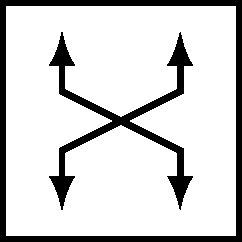
\includegraphics[width=0.9cm]{../common/fig-switch.pdf}
}
\providecommand{\router}{%
    
\includegraphics[width=0.9cm]{../common/fig-router.pdf}
}
\begin{frame}{switch v router: tables}
\begin{tikzpicture}
\matrix[tight matrix,
    nodes={minimum height=.6cm},
    column 1/.style={nodes={text width=5cm,font=\small\tt}},
    column 2/.style={nodes={text width=1cm,font=\small\tt}},
    row 1/.style={nodes={font=\small}},
    label={north:switch (`bridge') table},
] (bridge table) {
MAC address \& port \\
00:11:22:33:44:55 \& 1 \\
00:33:00:01:02:aa \& 2 \\
00:44:00:01:02:bb \& 3 \\
\ldots \& \ldots \\
};
\matrix[tight matrix,
    nodes={minimum height=.6cm},
    column 1/.style={nodes={text width=4.5cm,font=\small\tt}},
    column 2/.style={nodes={text width=2cm,font=\small\tt,alt=<4>{fill=red!10}}},
    column 3/.style={nodes={text width=1cm,font=\small\tt,alt=<3>{fill=red!10}}},
    row 1/.style={nodes={font=\small}},
    label={north:routing table},
    anchor=north west
] (route table) at ([xshift=.5cm]bridge table.north east){
IP addresses \& gateway \& iface \\
2001:0db8:40::/48 \& --- \& int \\
3fff:1000:19::/48 \& --- \& ext \\
\ldots \& \ldots \& \ldots \\
\normalfont default \& fe80::17 \& ext \\
};
\begin{visibleenv}<2>
\node[
    draw=red,ultra thick,fit=(bridge table),
] (bridge table around) {};
\node[align=left,anchor=north west] at (bridge table around.south west) {
    one logical device with multiple ports \\
    not in table: always broadcast
};
\end{visibleenv}
\begin{visibleenv}<3->
\node[
    draw=red,ultra thick,fit=(route table),
] (route table around) {};
\end{visibleenv}
\begin{visibleenv}<3>
\node[align=left,anchor=north] at (route table around.south) {
    `interface' = which network \\
    ~ \\
    one interface might have multiple ports \\
    that are `bridged' together \\
};
\end{visibleenv}
\begin{visibleenv}<4>
\node[align=left,anchor=north] at (route table around.south) {
    gateway = who to send to next \\
    no gateway = `direct' to destination \\
    ~ \\
    need to have specific destination \\
    to send to on interface
};
\end{visibleenv}
\end{tikzpicture}
\end{frame}

\begin{frame}{switch v router: on the wires}
\begin{tikzpicture}
\tikzset{
    computer/.style={inner sep=0mm,outer sep=0mm,execute at begin node={\computer}},
    switch/.style={inner sep=0mm,outer sep=0mm,execute at begin node={\switch}},
    router/.style={inner sep=-1mm,outer sep=0mm,execute at begin node={\router},circle},
    connect/.style={draw,very thick,Latex-Latex},
    connect big/.style={draw,ultra thick,Latex-Latex},
    addr label/.style={align=left,font=\fontsize{9}{10}\selectfont\tt},
}w
\node[computer,label={[addr label]south:MAC 00:\ldots:AA\\IP 10.0.1.2},alt=<5>{draw=red,ultra thick,fill=red!10}] (n1-c1) at (0, -2.5) {};
\node[computer,label={[addr label]south:MAC 04:\ldots:BB\\IP 10.0.1.3}]  (n1-c2) at (0, 0) {};
\node[switch] (n1-s1) at (3,-1) {};
\node[switch] (n1-s2) at (5,-4) {};
\node[computer,label={[addr label]south:MAC 05:\ldots:CC\\IP 10.0.1.4}] (n1-c3) at (1, -5) {};
\draw[connect] (n1-c1) -- (n1-s1);
\draw[connect] (n1-c2) -- (n1-s1);
\draw[connect] (n1-c3) -- (n1-s2);
\draw[connect big] (n1-s1) -- (n1-s2);
\node[router,label={[addr label]south:MAC \myemph<5-6>{02:\ldots:DD} / 02:\ldots:DE\\IP: 10.0.1.1 / 10.0.2.15},alt=<5-6>{fill=red!10,draw=red,ultra thick}] (n1n2) at (9, -5) {};
\node[switch] (n2-s1) at (11, -3) {};
\node[computer,label={[addr label]south:MAC 03:\ldots:EE\\IP: \myemph<5>{10.0.2.2}},alt=<5>{draw=red,ultra thick,fill=red!10}] (n2-c1) at (12.5, -4) {};
\draw[connect](n2-s1) -- (n2-c1);

\draw[connect big] (n1-s2) -- (n1n2);
\draw[connect big] (n2-s1) -- (n1n2);
\begin{pgfonlayer}{bg}
    \begin{visibleenv}<2->
        \path[overlay,draw=violet,fill=violet!10]
            (-1.3, -7) -- (5, -7) -- (9, -7) -- (9, -3) -- (4, .75) -- (-1.3, .75) -- cycle;
        \path[overlay,draw=green,fill=green!10]
            (7, 0) -- (8, -2) -- (9, -3) -- (9, -7) -- (13.5, -7) -- (13.5, 0) -- cycle;
        \node[anchor=south,font=\tt] at (5, -7) {10.0.1.0/24};
        \node[anchor=south,font=\tt] at (11, -7) {10.0.2.0/24};
    \end{visibleenv}
\end{pgfonlayer}
\begin{visibleenv}<3->
        \foreach \x [remember=\x as \lastx (initially n1-c1)] in {n1-s1,n1-s2,n1n2,n2-s1,n2-c1} {
            \path[draw,dotted,blue,line width=1mm,arrows=-Latex] (\lastx) -- (\x);
        }
\end{visibleenv}
\begin{visibleenv}<4->
    \path[draw,blue,thick] ($(n1-c1)!0.5!(n1-s1)$) -- (3.7, -1) ++ (0, 1.) coordinate (n1 frame base);
    \node[font=\fontsize{9}{10}\tt,anchor=north west] (n1 outer) at (n1 frame base) {
        00:\ldots:AA\hspace{1mm}$\rightarrow$\myemph<5>{\hspace{1mm}02:\ldots:DD}
    };
    \node[align=left,font=\fontsize{9}{10}\tt,anchor=north west,draw=black!50,very thick,
          alt=<6>{fill=red!10},
    ] (n1 inner) at ([xshift=1mm]n1 outer.south west) {
        10.0.1.3 $\rightarrow$ \myemph<5>{10.0.2.2} \\
        (actual data)
    };
    \path (12, -0) ++ (-2.25, 0.5) coordinate (n2 frame base);
    \node[font=\fontsize{9}{10}\tt,anchor=north west] (n2 outer) at (n2 frame base) {
        02:\ldots:DE\hspace{1mm}$\rightarrow$\hspace{1mm}03:\ldots:EE
    };
    \node[align=left,font=\fontsize{9}{10}\tt,anchor=north west,draw=black!50,very thick,
          alt=<6>{fill=red!10}
    ] (n2 inner) at ([xshift=1mm]n2 outer.south west) {
        10.0.1.3 $\rightarrow$ 10.0.2.2 \\
        (actual data)
    };
\end{visibleenv}
\begin{pgfonlayer}{bg}
    \begin{visibleenv}<4->
    \node[inner sep=0mm,fill=white,draw=blue,very thick,
          fit={(n1 outer) (n1 inner) ([yshift=-1mm]n1 inner.south) ([xshift=1mm]n1 inner.east)}
    ] (n1 box) {};
    \path[draw,blue,thick] ($(n1-s1)!0.5!(n1-s2)$) -- (n1 box);
    \path[draw,blue,thick] ($(n1-s2)!0.5!(n1n2)$) -- (n1 box);
    \node[inner sep=0mm,fill=white,draw=blue,very thick,
          fit={(n2 outer) (n2 inner) ([yshift=-1mm]n2 inner.south) ([xshift=1mm]n2 inner.east)}
    ] (n2 box) {};
    \path[draw,blue,thick] ($(n2-s1)!0.5!(n1n2)$) -- ([xshift=.5cm]n2 box.south west);
    \path[draw,blue,thick] ($(n2-c1)!0.5!(n2-s1)$) -- ([xshift=2cm]n2 box.south west);
    \end{visibleenv}
\end{pgfonlayer}
\begin{visibleenv}<5>
    \node[fill=white,draw=red,ultra thick,align=left] at (3, -5) {
        MAC address = on \textit{local} network \\
        IP address = somewhere else
    };
\end{visibleenv}
\begin{visibleenv}<7>
    \draw[red, ultra thick] (n1 inner) -- (n2 inner)
        node[inner sep=0mm,
             midway,pin={[pin edge={red,ultra thick},fill=white,draw=red,thick,align=center]-90:IP packet copied as is\\placed in new frame}] {};
\end{visibleenv}
% FIXME:    show packets involved
% FIXME:    show frames involved
% FIXME:    show bridge/routing table
\end{tikzpicture}
\end{frame}

\begin{frame}{the view from the source}
\begin{tikzpicture}
\tikzset{
    computer/.style={inner sep=0mm,outer sep=0mm,execute at begin node={\computer}},
    switch/.style={inner sep=0mm,outer sep=0mm,execute at begin node={\switch}},
    router/.style={inner sep=-1mm,outer sep=0mm,execute at begin node={\router},circle},
    connect/.style={draw,very thick,Latex-Latex},
    connect big/.style={draw,ultra thick,Latex-Latex},
    addr label/.style={align=left,font=\fontsize{9}{10}\selectfont\tt},
}w
\node[computer,label={[addr label]south:MAC 00:\ldots:AA\\IP 10.0.1.2},alt=<5>{draw=red,ultra thick,fill=red!10}] (n1-c1) at (0, -2.5) {};
\node[computer,label={[addr label]south:MAC 04:\ldots:BB\\IP 10.0.1.3}]  (n1-c2) at (0, 0) {};
\node[switch] (n1-s1) at (3,-1) {};
\node[switch] (n1-s2) at (5,-4) {};
\node[computer,label={[addr label]south:MAC 05:\ldots:CC\\IP 10.0.1.4}] (n1-c3) at (1, -5) {};
\draw[connect] (n1-c1) -- (n1-s1);
\draw[connect] (n1-c2) -- (n1-s1);
\draw[connect] (n1-c3) -- (n1-s2);
\node[router,label={[addr label]south:MAC \myemph<5-6>{02:\ldots:DD} / 02:\ldots:DE\\IP: 10.0.1.1 / 10.0.2.15},alt=<5-6>{fill=red!10,draw=red,ultra thick}] (n1n2) at (9, -5) {};
\draw[connect big] (n1-s1) -- (n1-s2);
\draw[connect big] (n1-s2) -- (n1n2);

% FIXME: network diagram without second network
    % show packet generated
% FIXME: routing table for 10.0.1.2
% FIXME: show application asking to send packet
% FIXME: ask Q of how we know destination MAC field
% FIXME: show ARP table
\end{tikzpicture}
\end{frame}
